\section{Interfaces}

\begin{figure}
  \centering
  \begin{subfigure}[b]{0.22\textwidth}
    \fbox{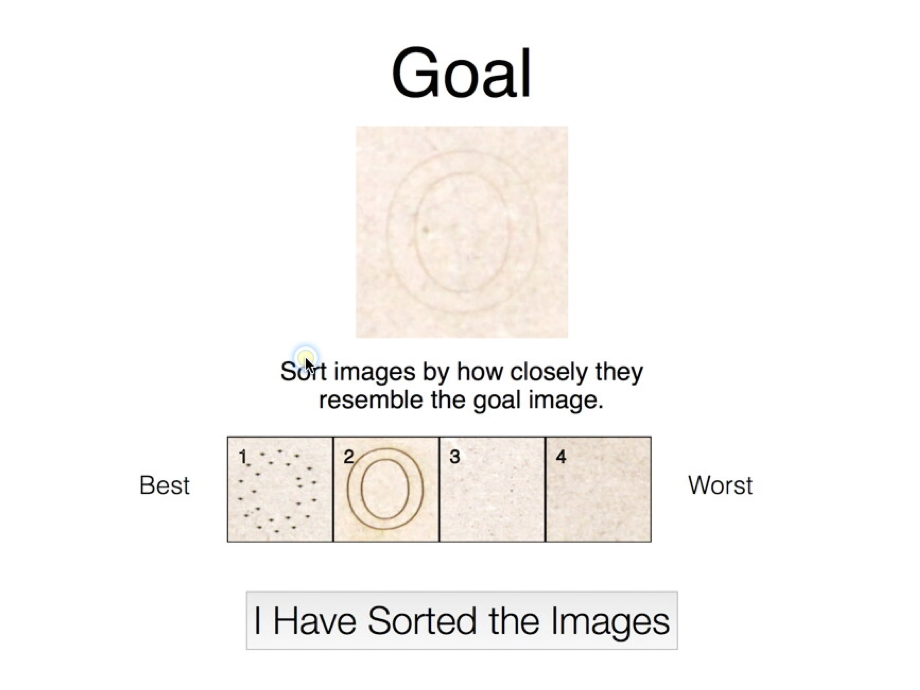
\includegraphics[width=\textwidth]{figures/interface_nm}}
    \caption{Nelder-Mead}\label{fig:interface_nm}
  \end{subfigure}
  \quad
  \begin{subfigure}[b]{0.22\textwidth}
    \fbox{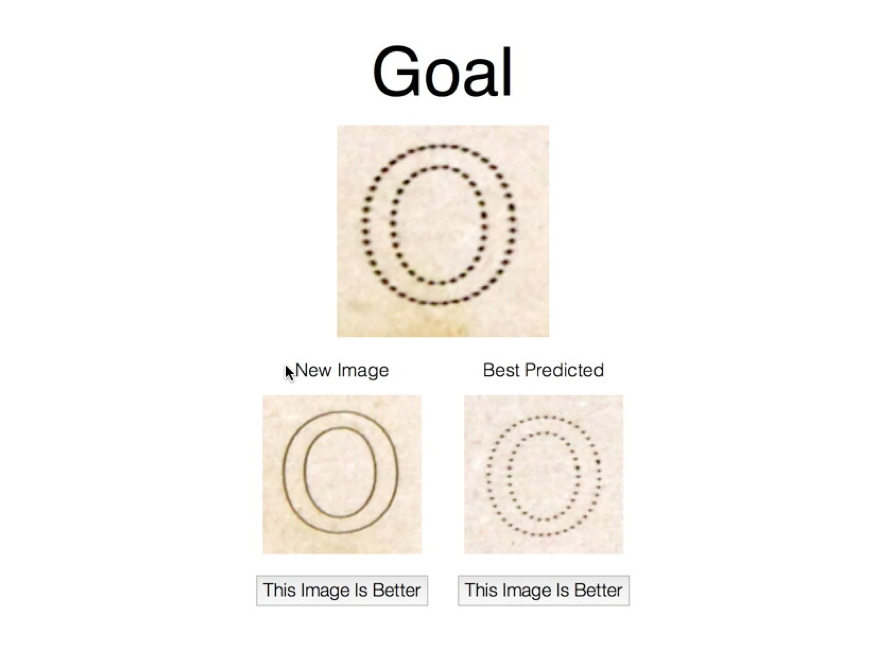
\includegraphics[width=\textwidth]{figures/interface_bo}}
    \caption{Bayesian Optimization}\label{fig:interface_bo}
  \end{subfigure}
  \caption{Interaces to the optimization algorithms.}\label{fig:interfaces}
\end{figure}

\subsection{Nelder-Mead Rank Sorting Interface}

When choosing how to move the worst point, the Nelder-Mead algorithm may need to know any of the following:
the worst vertex, the best vertex, or the second-to-worst vertex.
All of these can be collected at once.
The current interface (see Figure~\ref{fig:interface_nm}) asks a user to produce a ranked list of the vertices from best to worst.
They can do this by clicking and dragging examples to put the best examples at the front of the queue.

When a user finishes ranking, they click a button.
The simplex chooses candidate next points.
If the algorithm needs clarification about candidate points (e.g., to determine if an expansion is better than a reflection), it inserts them into the list.
The user ranks them among the original vertices to resolve the ambiguity.
Once it replaces the worst point, the list is cleaned to show only the simplex's four current vertices.

\subsection{Bayesian Optimization Pair Comparison Interface}

With Brochu et al.'s variant on Bayesian optimization~\cite{brochu_tutorial_2010}, an optimal point for a cost function that's expensive to evaluate can be found by collecting comparison ratings between pairs of examples.
In their interface, a user was shown the best example so far, and an examples that maximized expected improvement.
The user was prompted to make a choice about which of the two was better.

My interface for Bayesian Optimization is very similar to Brochu et al.'s (see Figure~\ref{fig:interface_bo}).
A user is shown the best rated example, and an example that maximizes the expected improvement.
With each rating, both the best rated example and that which maximizes expected improvement are updated.

Both interfaces show the goal configuration at the top-center to guide users' exploration during the experiments.
